% =====================================================================
%  ST7072CEM Machine Learning: LoRa propagation and ML path loss modelling, Nepal hills
%  Compile with pdflatex. Figures and photos are expected in ./figures/
% =====================================================================
\documentclass[conference]{IEEEtran}
\IEEEoverridecommandlockouts

\usepackage{cite}
\usepackage{amsmath,amssymb}
\usepackage{graphicx}
\usepackage{booktabs}
\usepackage{array}
\usepackage{xcolor}
\usepackage{url}
\usepackage{xspace}
\usepackage{subcaption}
\usepackage{float}
\usepackage[hidelinks]{hyperref}

\graphicspath{{figures/}}
\newcommand{\dBm}{\,dBm\xspace}
\newcommand{\dB}{\,dB\xspace}
\newcommand{\photo}[1]{\IfFileExists{figures/#1}{\includegraphics[height=4.0cm]{figures/#1}}{\IfFileExists{#1}{\includegraphics[height=4.0cm]{#1}}{\fbox{\parbox[c][3.6cm][c]{0.85\linewidth}{\centering\footnotesize photo missing:\\\texttt{\detokenize{#1}}}}}}}

\begin{document}

\title{Experimental Characterization of LoRa Propagation and Machine Learning Approaches for Path Loss Modeling Across Diverse Hill Terrains in Nepal}

\author{\IEEEauthorblockN{Peter Karki}
\IEEEauthorblockA{\textit{ST7072CEM Machine Learning}\\
\textit{Softwarica College of IT and E-Commerce}\\
Coventry ID: 17624929\\
260054@softwarica.edu.np}
}

\maketitle

% ---------------------------------------------------------------------
\begin{abstract}
LoRa could support sensing in Nepal's hills, but most path loss models come from flat or urban areas. We built a two-node 866\,MHz instrument that, at each stop, sweeps six spreading factors (SF7--SF12) and three transmit powers (2, 8 and 14\dBm) with five packets each, and collected 61 complete sweeps (5,490 packet slots) in three hill-terrain case studies near Kathmandu. Models were validated grouped by stop and by leaving out a whole case. A depth-3 decision tree using only spreading factor and power predicted delivery with a balanced accuracy of 0.68, and 0.67 on an unseen case. Path loss was not predictable from distance or endpoint terrain features: no model beat the mean-only baseline (RMSE 11.1\dB), and a log-distance fit held only in the short-range case ($n = 2.10$). The cheapest setting delivering four of five packets needed a median 97\% less transmit energy than SF12 at 14\dBm. An interactive dashboard maps predicted dead zones on example terrain. In hill terrain, what lies between the antennas matters more than the distance between them.
\end{abstract}

\begin{IEEEkeywords}
LoRa, path loss, machine learning, hill terrain, grouped cross-validation, Nepal
\end{IEEEkeywords}

% ---------------------------------------------------------------------
\section{Introduction}

LoRa is a long-range, low-power radio widely used for Internet of Things (IoT) sensing. In Nepal's hills it could support agriculture and hazard monitoring where cellular coverage is patchy. Planning such networks needs an estimate of path loss, usually from the log-distance model, in which loss grows with the logarithm of distance~\cite{rappaport2002}. Its parameters, however, come mostly from flat or urban areas. In hills, two points a few hundred metres apart may be separated by a ridge, while points kilometres apart across a valley may see each other clearly. Planners therefore rely on trial and error, and field data from such terrain are scarce for Nepal.

Machine learning (ML) can add terrain information to path loss prediction, but two problems limit how far published results transfer: few studies cover hill terrain in South Asia, and random train--test splits can put measurements from the same place in both sets and overstate accuracy. We therefore built an instrument that tests every combination of six spreading factors and three transmit powers at each stop, which separates the effect of radio settings from that of location, and measured three contrasting case studies (Table~\ref{tab:caseintro}). The research questions are:
\begin{itemize}
    \item \textbf{RQ1:} Do distance and simple terrain features improve path loss prediction over log-distance or mean-only baselines?
    \item \textbf{RQ2:} Do models trained in some terrain cases transfer to a different case?
    \item \textbf{RQ3:} What is the cheapest radio setting each location needs?
\end{itemize}

\begin{table}[t]
\caption{The three case studies}\label{tab:caseintro}
\centering
\footnotesize
\setlength{\tabcolsep}{3pt}
\begin{tabular}{@{}l>{\raggedright\arraybackslash}p{0.75cm}>{\raggedright\arraybackslash}p{3.0cm}>{\raggedright\arraybackslash}p{1.35cm}c@{}}
\toprule
Case & Site & Setting & Range & Stops \\
\midrule
1 & A & Forested slope; Station antenna 2.0\,m & 22--250\,m & 17 \\
2 & B & Hill slope across a valley; antenna 1.0\,m & 0.2--2.9\,km & 36 \\
3 & C, D & Town rooftops ($\approx$9 and 6\,m) & 0.3--3.3\,km & 8 \\
\bottomrule
\end{tabular}
\end{table}

The contributions are:
\begin{enumerate}
    \item a reproducible two-node instrument that records delivery, RSSI and SNR for 18 radio configurations at every stop, and a dataset of 61 complete sweeps in three hill-terrain cases;
    \item an evaluation of regression, decision-tree and ensemble models against simple baselines, using validation grouped by stop and a leave-one-case-out test;
    \item evidence that radio settings transfer between terrains while distance-based path loss does not, an explanation of why, and the cheapest working setting at each stop;
    \item an interactive dashboard that presents the results and maps predicted dead zones on example terrain.
\end{enumerate}
Table~\ref{tab:abbr} lists the abbreviations used.

\begin{table}[t]
\caption{Abbreviations}\label{tab:abbr}
\centering
\footnotesize
\setlength{\tabcolsep}{4pt}
\begin{tabular}{@{}ll@{}}
\toprule
Abbreviation & Full form \\
\midrule
AP / AUC & Average precision / area under the ROC curve \\
IoT & Internet of Things \\
GPS & Global Positioning System \\
LiDAR & Light detection and ranging \\
LOCO / LOO & Leave-one-case-out / leave-one-stop-out \\
OLS & Ordinary least squares \\
LoRa & Long Range (radio modulation) \\
LPWAN & Low-power wide-area network \\
ML & Machine learning \\
NOACK & No acknowledgement (handshake failed) \\
PL & Path loss \\
RF & Random forest \\
RMSE & Root-mean-square error \\
ROC & Receiver operating characteristic \\
RQ & Research question \\
RSSI / SNR & Received signal strength / signal-to-noise ratio \\
SF & Spreading factor \\
SRTM & Shuttle Radar Topography Mission \\
\bottomrule
\end{tabular}
\end{table}

% ---------------------------------------------------------------------
\section{Literature Review}\label{sec:related}

\subsection{Classical path loss models}
The log-distance model fits a path loss exponent $n$ and a shadowing term to measurements~\cite{rappaport2002}. The Okumura--Hata model adds corrections for frequency and antenna heights, but assumes base stations above 30\,m and distances over 1\,km~\cite{hata1980}, and diffraction models such as ITU-R P.526 estimate the extra loss over hills~\cite{itu_p526}. At 866\,MHz these models differ by more than 40\dB at 1\,km, and none follows the spread of our stops (Fig.~\ref{fig:litmodels}).

\begin{figure}[t]
\centering
\includegraphics[width=\columnwidth]{fig_lit_models.png}
\caption{Classical path loss models at 866\,MHz with this study's 60 stops (grey). Drawn by the author from the published equations.}
\label{fig:litmodels}
\end{figure}

\subsection{Empirical LoRa measurements}
Petäjäjärvi \textit{et al.}~\cite{petajajarvi2015} measured LoRa at 868\,MHz in Oulu, Finland, and reported ranges over 15\,km on flat ground and about 30\,km over water at SF12 and 14\dBm (Fig.~\ref{fig:card-petajajarvi}). They also derived a channel attenuation model for similar flat areas.

\begin{figure}[H]
\centering
\includegraphics[width=\columnwidth]{card_petajajarvi.png}
\caption{Conceptual summary of~\cite{petajajarvi2015}: maximum range with one setting in flat terrain. Drawn by the author.}
\label{fig:card-petajajarvi}
\end{figure}

Rademacher \textit{et al.}~\cite{rademacher2021} collected over 112,000 samples during 230 days in a 200\,km$^2$ urban area and compared eleven models. Log-distance, Okumura and Winner+ gave reasonable estimates, whereas terrain-based models gave no gain (Fig.~\ref{fig:card-rademacher}).

\begin{figure}[H]
\centering
\includegraphics[width=\columnwidth]{card_rademacher.png}
\caption{Conceptual summary of~\cite{rademacher2021}: eleven empirical models compared in a city. Drawn by the author.}
\label{fig:card-rademacher}
\end{figure}

In an Alpine canyon, Bianco \textit{et al.}~\cite{bianco2020} measured 868\,MHz LoRa with a single setting (SF7, 14\dBm) and reached only about 300\,m at 50\% delivery, far less than on flat ground (Fig.~\ref{fig:card-bianco}).

\begin{figure}[H]
\centering
\includegraphics[width=\columnwidth]{card_bianco.png}
\caption{Conceptual summary of~\cite{bianco2020}: range at 50\% delivery in an Alpine canyon. Drawn by the author.}
\label{fig:card-bianco}
\end{figure}

In Nepal, Pokharel \textit{et al.}~\cite{pokharel2024} recommended settings from one 433\,MHz link of about 5\,km, without ML (Fig.~\ref{fig:card-pokharel}). All four studies used one link or one radio setting at a time, which motivates multi-configuration measurements at many locations.

\begin{figure}[H]
\centering
\includegraphics[width=\columnwidth]{card_pokharel.png}
\caption{Conceptual summary of~\cite{pokharel2024}: one long link in Nepal used to recommend settings. Drawn by the author.}
\label{fig:card-pokharel}
\end{figure}

\subsection{Machine learning for path loss}
Ojo \textit{et al.}~\cite{ojo2024} fed the sequence of land-cover classes along each link to a bidirectional LSTM and reported a mean error of 4.97\dB from over 35,000 packets of sheep-tracking devices on Alpine pastures, about half the error of established empirical models (Fig.~\ref{fig:card-ojo}).

\begin{figure}[H]
\centering
\includegraphics[width=\columnwidth]{card_ojo.png}
\caption{Conceptual summary of~\cite{ojo2024}: a sequence model using land cover along the path. Drawn by the author.}
\label{fig:card-ojo}
\end{figure}

Ethier and Châteauvert~\cite{ethier2024} showed, on 8.2 million measurements, that adding obstacle depth along the path cut the median RMSE by about 5\dB, to 7.5\dB (Fig.~\ref{fig:card-ethier}).

\begin{figure}[H]
\centering
\includegraphics[width=\columnwidth]{card_ethier.png}
\caption{Conceptual summary of~\cite{ethier2024}: median RMSE over six held-out cities. Drawn by the author.}
\label{fig:card-ethier}
\end{figure}

Bitterling \textit{et al.}~\cite{bitterling2026} found that random forests~\cite{breiman2001} with LiDAR terrain features beat baselines under random splits but degraded when whole gateways were held out (Fig.~\ref{fig:card-bitterling}). Together these works suggest that terrain \emph{along the path} is informative and that validation design strongly affects reported accuracy. Decision trees~\cite{breiman1984} remain attractive for small datasets because their rules can be read and checked.

\begin{figure}[H]
\centering
\includegraphics[width=\columnwidth]{card_bitterling.png}
\caption{Conceptual summary of~\cite{bitterling2026}: the verdict changes with the validation design. Drawn by the author.}
\label{fig:card-bitterling}
\end{figure}

\subsection{Censoring and validation}
Weak links are lost rather than measured, so ignoring them biases the fitted exponent; a Tobit estimator~\cite{tobin1958} corrects this~\cite{gustafson2015} (Fig.~\ref{fig:card-gustafson}). Samples grouped in space also make random cross-validation optimistic~\cite{roberts2017}; packets from one stop form such a group. LoRa data are strongly affected by both issues because many packets are lost at long range and each location yields many packets.

\subsection{Why the reported metrics are not benchmarks}
The studies answer different questions with different data: maximum range, delivery at one setting, mean error of a sequence model, or RMSE over held-out cities. Their frequencies, sample sizes, targets and validation schemes differ, so their numbers describe the field but cannot be ranked against each other or against this study. Table~\ref{tab:compare} therefore keeps each metric in its original form.

\begin{figure}[H]
\centering
\includegraphics[width=\columnwidth]{card_gustafson.png}
\caption{Conceptual summary of~\cite{gustafson2015}: ignoring lost samples biases the fitted exponent. Drawn by the author.}
\label{fig:card-gustafson}
\end{figure}

\begin{table*}[t]
\caption{Comparable studies (metrics in original form; not directly comparable)}\label{tab:compare}
\centering
\footnotesize
\setlength{\tabcolsep}{4pt}
\begin{tabular}{@{}>{\raggedright\arraybackslash}p{2.7cm}>{\raggedright\arraybackslash}p{3.3cm}>{\raggedright\arraybackslash}p{3.3cm}>{\raggedright\arraybackslash}p{3.6cm}>{\raggedright\arraybackslash}p{3.3cm}@{}}
\toprule
Study & Setting & Method & Result & Limitation here \\
\midrule
Petäjäjärvi~\cite{petajajarvi2015} & Flat land and sea & SF12, 14\dBm & $>$15\,km, $\approx$30\,km & Flat; one setting \\
Rademacher~\cite{rademacher2021} & Urban, 112k samples & 11 empirical models & Log-distance adequate & City; no ML \\
Bianco~\cite{bianco2020} & Alpine canyon & SF7, 14\dBm & $\approx$300\,m at 50\% & One setting \\
Pokharel~\cite{pokharel2024} & Nepal, 433\,MHz & One link & Settings advice & Single link \\
Ojo~\cite{ojo2024} & Alpine pastures & Bi-LSTM, land cover & 4.97\dB mean error & Large dataset \\
Ethier~\cite{ethier2024} & UK drive tests & ML, obstacle depth & RMSE $\approx$7.5\dB & Urban, 8.2M samples \\
Bitterling~\cite{bitterling2026} & LPWAN gateways & RF + LiDAR & Drops on new gateways & -- \\
\textbf{This work} & Nepal hills, 61 stops & Trees, ridge, Tobit, RF & 0.67 on unseen case & -- \\
\bottomrule
\end{tabular}
\end{table*}

\subsection{Research gap}
No reviewed study combines multi-setting LoRa measurements in Himalayan foothills, explicit handling of censored and failed links, and ML validation that holds out whole terrain cases (Table~\ref{tab:gap}). This study is small, so it does not aim to outperform the reviewed work; it tests whether their approaches hold in a new setting.

\begin{table}[t]
\caption{Research gaps}\label{tab:gap}
\centering
\footnotesize
\setlength{\tabcolsep}{3pt}
\begin{tabular}{@{}>{\raggedright\arraybackslash}p{1.6cm}>{\raggedright\arraybackslash}p{3.1cm}>{\raggedright\arraybackslash}p{3.0cm}@{}}
\toprule
Gap & Prior work & This study \\
\midrule
Terrain & Flat, urban, Alpine~\cite{petajajarvi2015,rademacher2021,bianco2020} & Three Nepal hill cases \\
Settings & One per campaign~\cite{bianco2020} & 18 per stop \\
Censoring & Rarely handled~\cite{gustafson2015} & Tobit; 30 lost locations \\
Validation & Random splits~\cite{bitterling2026} & By stop and by case \\
\bottomrule
\end{tabular}
\end{table}

% ---------------------------------------------------------------------
\section{Measurement Setup and Data}\label{sec:data}

\subsection{LoRa background}
LoRa uses chirp spread spectrum~\cite{semtech_an1200,augustin2016}. Each step from SF7 to SF12 doubles airtime and lowers the SNR needed for decoding by about 2.5\dB, down to about $-20$\dB at SF12. A higher SF therefore trades airtime and energy for range, and links can survive below the thermal noise floor. Each extra decibel of transmit power adds one decibel at the receiver. Testing every SF--power pair at one place shows how much margin a link has.

\subsection{Instrument}
Both nodes use an ESP32 and an Ai-Thinker Ra-08H module at 866.1\,MHz and 125\,kHz, inside the band Nepal assigns to IoT~\cite{nta2023} (Figs.~\ref{fig:hwinfo} and~\ref{fig:instrument}). The fixed \textit{Station} transmits; the walking \textit{Roamer} receives and logs every slot with RSSI, SNR and GPS position (5--10\,m accuracy). Custom radio firmware was written because the vendor firmware cannot change SF and power directly; it was frozen for all measurements and fingerprinted with SHA-256 so any change would be detectable. The Roamer firmware (version 4.6.0) logs every slot to a CSV file on a microSD card. Antenna gains and cable losses were not measured.

\begin{figure*}[!t]
\centering
\includegraphics[width=\textwidth]{fig_hardware_info.png}
\caption{Hardware of the two-node instrument and its two radio links.}
\label{fig:hwinfo}
\end{figure*}

\begin{figure*}[t]
\centering
\begin{subfigure}[t]{0.32\textwidth}\centering\photo{station.jpg}\caption{Station}\end{subfigure}\hfill
\begin{subfigure}[t]{0.32\textwidth}\centering\photo{roamer.jpg}\caption{Roamer}\end{subfigure}\hfill
\begin{subfigure}[t]{0.32\textwidth}\centering\photo{field.jpg}\caption{Roamer in the field}\end{subfigure}
\caption{The instrument and its use in the field.}
\label{fig:instrument}
\end{figure*}

\subsection{Sweep protocol}
At each stop the Roamer requests a sweep over a control link (SF12, 14\dBm). The Station then sends five packets for each of 18 configurations, 90 slots in about 67\,s, each logged as OK or TIMEOUT (Table~\ref{tab:sweep}, Fig.~\ref{fig:sweep}). If the handshake fails (NOACK), no sweep runs, and the place is recorded as a failed attempt. In the Case~1 logs, sweeps after strong handshakes started 3.5--7\,s later and sweeps after weak handshakes 11--46\,s later, consistent with link margin rather than a clock fault.

\begin{table}[t]
\caption{Sweep configuration}\label{tab:sweep}
\centering
\footnotesize
\begin{tabular}{@{}ll@{}}
\toprule
Parameter & Value \\
\midrule
Frequency / bandwidth & 866.1\,MHz / 125\,kHz \\
Spreading factor & SF7--SF12 \\
Transmit power & 2, 8, 14\dBm \\
Packets per setting & 5 (90 slots per stop) \\
Control link & SF12, 14\dBm \\
\bottomrule
\end{tabular}
\end{table}

\begin{figure}[!t]
\centering
\includegraphics[width=\columnwidth]{fig_sweep_timeline.png}
\caption{One stop, step by step.}
\label{fig:sweep}
\end{figure}

\subsection{Data and cleaning}
The raw data are one Roamer log per site. They were combined, and only complete sweeps were kept: 61 stops (17, 36 and 8 per case), 5,490 slots and 2,612 received packets (47.6\%). The 56 failed handshakes reduce to 30 unique \textit{lost locations} (3, 9 and 18 per case) after removing retries within 30\,m of a completed stop. An earlier Site A run on older firmware was excluded because delivery at the same spots differed markedly. A scripted pipeline rebuilds the stop table (61 rows) and packet table (5,490 rows) from the raw logs and reproduces every reported number.

% ---------------------------------------------------------------------
\section{Methodology}\label{sec:method}

\subsection{Workflow and problem formulation}
Fig.~\ref{fig:workflow} summarises the workflow. For stop $s$ and slot $k$ with configuration $c_k = (\mathrm{SF}_k, P_k)$, the targets are
\begin{align}
y_s &= \operatorname{median}\{PL_{s,k} : P_k = 14\,\mathrm{dBm},\ z_{s,k}=1\}, \\
z_{s,k} &= 1 \text{ if slot } k \text{ was received, else } 0, \\
c^{*}_s &= \arg\min_{c}\, \mathrm{cost}(c) \ \text{s.t.} \textstyle\sum_{k:c_k=c} z_{s,k} \ge 4,
\end{align}
with $PL = P_{tx} - \mathrm{RSSI}$ and $\mathrm{cost}(c) = 10^{P/10}\cdot 2^{\mathrm{SF}-7}$. Path loss $y_s$ is a regression target, delivery $z_{s,k}$ a classification target and $c^{*}_s$ the cheapest working setting (RQ3). Apparent path loss includes the unmeasured antenna gains. Only 14\dBm packets define $y_s$ because the measured power steps were larger than nominal; 60 stops have a value, as one Case~1 stop received nothing.

\begin{figure}[t]
\centering
\includegraphics[width=\columnwidth]{fig_workflow.png}
\caption{Research methodology workflow.}
\label{fig:workflow}
\end{figure}

\subsection{Features}
Distance from Station to stop was computed with the haversine formula. Ground elevations of stops and Stations came from the SRTM 30\,m elevation model~\cite{farr2007}, giving the elevation difference (stop minus Station) and the elevation angle between the antennas. Land cover around each stop was labelled from satellite imagery as forest, built-up, mixed or open (14, 12, 31 and 4 stops) and one-hot encoded with forest as the reference. The models use $\log_{10}$ distance. Station antenna height (one value per site) and a manual line-of-sight label (made with delivery visible) were excluded to avoid leakage.

\subsection{Models and why they were chosen}
Path loss is continuous, so it is a regression problem: a mean-only baseline; the log-distance model $PL(d) = PL_0 + 10\,n\log_{10} d + X_\sigma$; least squares and ridge regression with terrain features (ridge suits few, correlated features); a depth-3 regression tree; and a 300-tree random forest. A Tobit fit on all packets treats each lost packet as path loss above its measurable limit~\cite{tobin1958,gustafson2015}.

Delivery is yes/no, so it is a classification problem. Depth-3 trees~\cite{breiman1984} with at least 90 packets per leaf were the main classifier: receiver sensitivity behaves like a threshold, the rules are readable, no leaf can memorise one stop, and the model is small enough for a node. Baselines were the majority class and a link-budget rule, which predicts delivery when the transmit power minus the log-distance prediction exceeds the sensitivity of the spreading factor; a random forest~\cite{breiman2001}, logistic regression and gradient boosting tested whether more flexible models help. Its random-split score was also recorded to show the effect of leakage. Neural networks were not used: with 61 independent locations, extra capacity would mainly memorise stops, and the sequence models that work well~\cite{ojo2024} relied on tens of thousands of links.

\subsection{Validation and metrics}
Packets from one stop share location and terrain, so they are not independent~\cite{roberts2017}. If one stop's packets appeared in both training and test sets, a model could recognise the stop instead of learning a general relationship. Every split therefore keeps a stop together (Fig.~\ref{fig:validation}). Regression used leave-one-stop-out (LOO) and leave-one-case-out (LOCO); classifiers used 10-fold cross-validation grouped by stop and LOCO. Metrics were RMSE, balanced accuracy, precision, recall, $F_1$, AUC and average precision:
\begin{align}
\mathrm{RMSE} &= \sqrt{\tfrac{1}{N}\textstyle\sum_i (y_i-\hat{y}_i)^2}, \quad
F_1 = \tfrac{2PR}{P+R}, \\
\mathrm{BalAcc} &= \tfrac{1}{2}\left(\tfrac{TP}{TP+FN}+\tfrac{TN}{TN+FP}\right),
\end{align}
where $P = TP/(TP+FP)$ and $R = TP/(TP+FN)$. Balanced accuracy is the headline metric because it weighs lost and delivered packets equally (0.5 is chance). With three cases, LOCO results are indicative. Associations used Spearman's $\rho$ and differences between cases the Kruskal--Wallis test. Table~\ref{tab:settings} lists the settings; the analysis used Python and scikit-learn~\cite{pedregosa2011}.

\begin{figure}[!t]
\centering
\includegraphics[width=\columnwidth]{fig_validation.png}
\caption{Validation schemes and resulting balanced accuracy.}
\label{fig:validation}
\end{figure}

\begin{table}[!t]
\caption{Model settings}\label{tab:settings}
\centering
\footnotesize
\setlength{\tabcolsep}{3pt}
\begin{tabular}{@{}ll@{}}
\toprule
Model & Setting \\
\midrule
Ridge & 30 penalties, $10^{-2}$--$10^{3}$ \\
Regression tree & Depth 3, $\ge$5 stops per leaf \\
Delivery tree & Depth 3, $\ge$90 packets per leaf \\
Random forest & 300 trees \\
Tobit & L-BFGS-B; 300 bootstrap resamples \\
Threshold / seed & 0.5 / 0 \\
\bottomrule
\end{tabular}
\end{table}

\subsection{Computational complexity}
For $n$ samples and $d$ features, least squares costs $O(nd^2)$, a tree $O(d\,n\log n)$ to train and $O(\text{depth})$ to predict, a forest of $T$ trees $T$ times more, and Tobit $O(kn)$ for $k$ iterations. Training time, prediction time and model size were measured as medians of five single-thread runs on a 2.1\,GHz cloud machine. A depth-3 tree answers with at most three comparisons, which matters on a small node.

\subsection{Dashboard}
A Gradio dashboard (Appendix~\ref{app:dash}) shows the results, re-runs grouped validation live and maps the tree's predicted dead zones on synthetic hill terrain, beside a geometric line-of-sight layer that the model cannot see. The expected receiver sensitivity used for the instrument check is the thermal noise floor ($\approx -117$\dBm for 125\,kHz and a 6\dB noise figure) plus the LoRa SNR limit of each spreading factor~\cite{semtech_an1200}.

% ---------------------------------------------------------------------
\section{Results}\label{sec:results}

\subsection{Instrument and delivery}
The weakest received packets matched the expected sensitivity: $-124$\dBm at SF7 (expected $-124.5$) and $-134$\dBm at SF12 (expected $-137$) (Fig.~\ref{fig:inst}). The lowest SNRs ($-10$ to $-21$\dB) were within about 2.5\dB of the demodulation limits, so the radios behaved as specified. Raising power from 2 to 14\dBm raised the median RSSI at the same stop and SF by 15.3\dB, not the nominal 12\dB (8 to 14\dBm: 8\dB; 2 to 8\dBm: 7\dB), which supports using only 14\dBm packets for path loss. Delivery rose with SF and power in every case, from 16\% at SF7/2\dBm to 88\% at SF12/14\dBm (Fig.~\ref{fig:heat}). At SF12/14\dBm, delivery was 75\%, 92\% and 95\% in Cases 1--3. Case~1 delivered only 2\% at SF7/2\dBm, against 24\% in Case~2, consistent with heavy obstruction at short range. Most stops were neither fully connected nor disconnected, the regime in which configuration choices matter most. Differences between cases were not significant (Kruskal--Wallis $p = 0.18$ for delivery, $p = 0.34$ for path loss; Table~\ref{tab:cases}).

\begin{figure}[t]
\centering
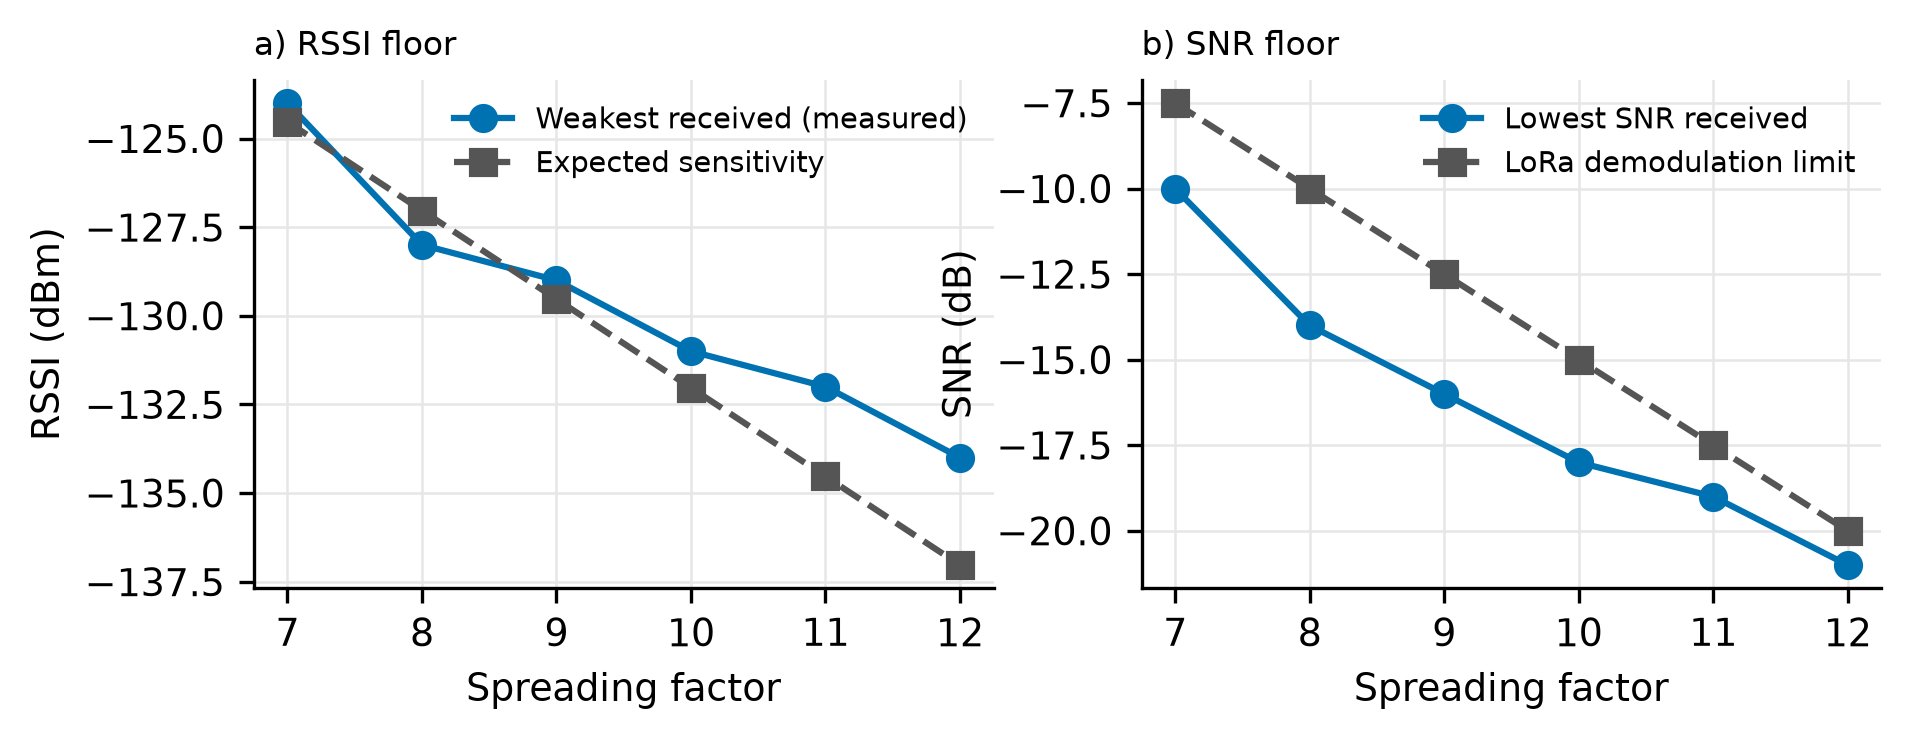
\includegraphics[width=\columnwidth]{fig7_sensitivity_check.png}
\caption{Weakest received RSSI and lowest SNR per SF against expected limits.}
\label{fig:inst}
\end{figure}

\begin{figure*}[t]
\centering
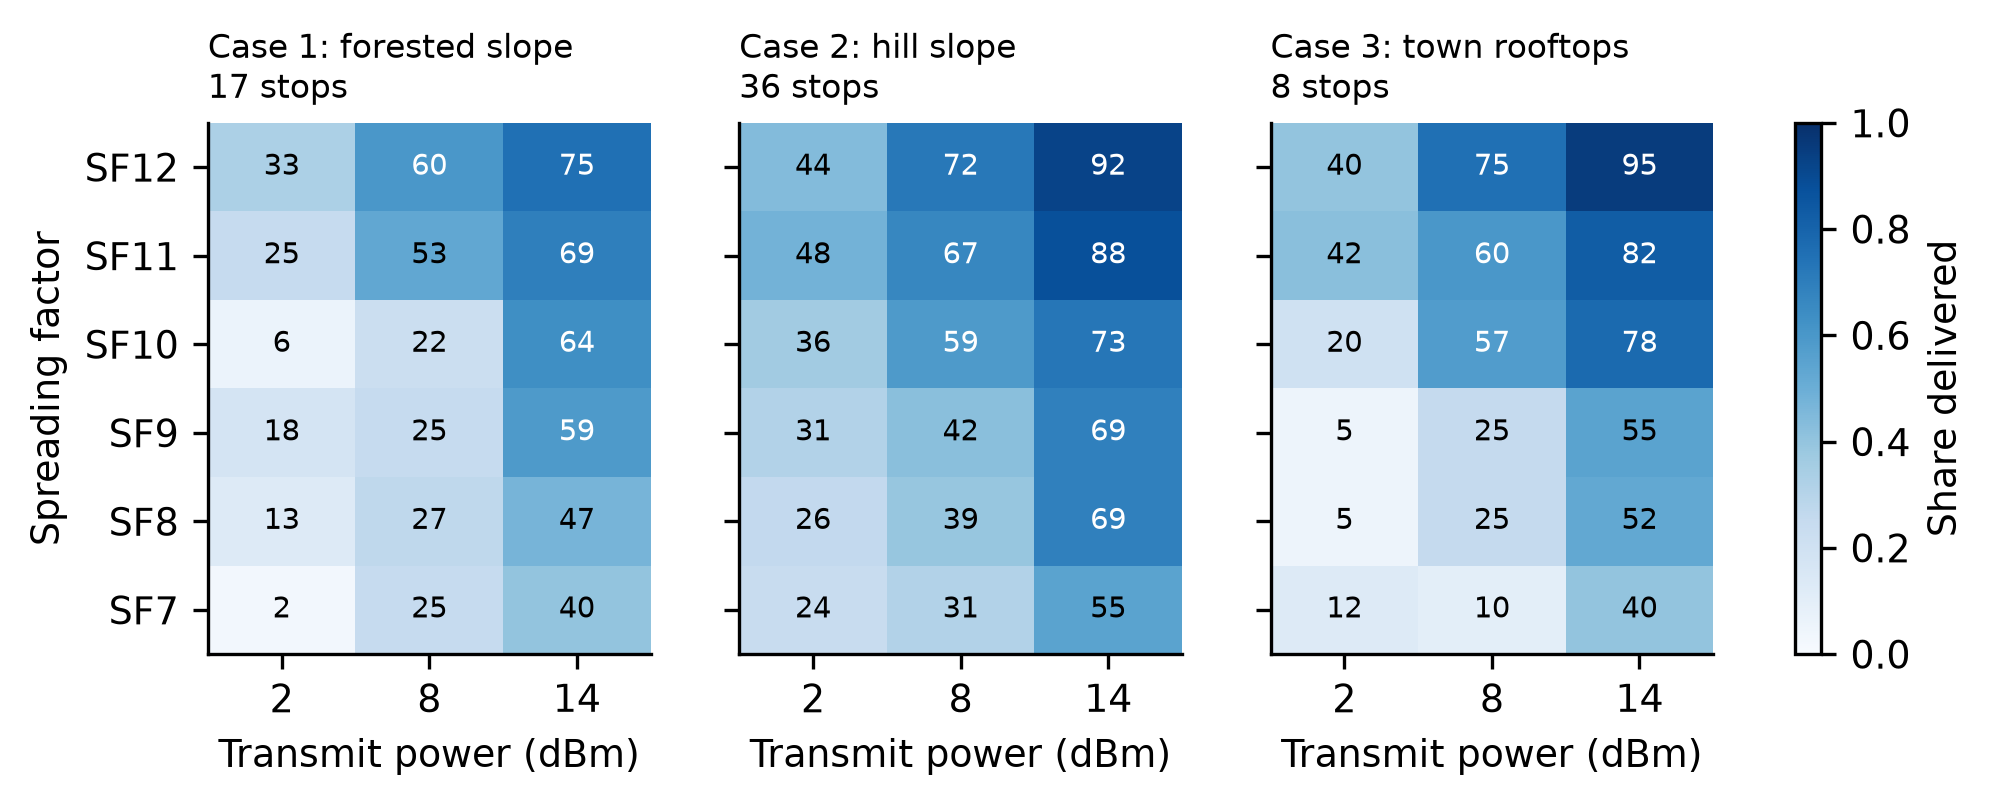
\includegraphics[width=0.82\textwidth]{fig2_delivery_by_case.png}
\caption{Share of packets delivered for each SF and transmit power, per case.}
\label{fig:heat}
\end{figure*}

\begin{table}[t]
\caption{Case-study profiles}\label{tab:cases}
\centering
\footnotesize
\setlength{\tabcolsep}{3.5pt}
\begin{tabular}{@{}lccc@{}}
\toprule
 & Case 1 & Case 2 & Case 3 \\
\midrule
Stops (sites) & 17 (A) & 36 (B) & 8 (C, D) \\
Median distance (m) & 185 & 1,374 & 2,248 \\
Distance range (m) & 22--250 & 209--2,916 & 272--3,268 \\
Elevation diff.\ (m) & 0 to 36 & $-34$ to 113 & $-4$ to 287 \\
Received / slots & 563/1,530 & 1,737/3,240 & 312/720 \\
Delivery (\%) & 36.8 & 53.6 & 43.3 \\
Median $PL_{14}$ (dB) & 129.5 & 130.0 & 134.0 \\
Lost locations & 3 & 9 & 18 \\
Link success (\%) & 85 & 80 & 31 \\
$\rho$(delivery, distance) & $-0.58^{*}$ & $-0.02$ & $-0.42$ \\
$\rho$(delivery, elev.\ diff.) & $-0.26$ & $0.49^{*}$ & $-0.04$ \\
\bottomrule
\multicolumn{4}{@{}l}{\scriptsize $^{*}p<0.05$.}
\end{tabular}
\end{table}

\subsection{Path loss, distance and link existence}
Pooled over 60 stops, path loss was nearly independent of distance ($n = 0.14$, 95\% CI $-0.44$ to 0.72, $\sigma = 11.1$\dB; Fig.~\ref{fig:pl}, Table~\ref{tab:fits}). Only Case~1 followed the expected trend ($n = 2.10$, $R^2 = 0.41$). Case~2 showed no trend, with path loss at similar distances ranging from about 100 to 145\dB, and the Case~3 fit rests on eight stops with a confidence interval that includes zero. The censoring-aware Tobit fit was also flat ($n = -0.12$, CI $-1.12$ to 0.64). Delivery rose with the stop's elevation above the Station ($\rho = 0.33$, $p = 0.008$), driven by Case~2 ($\rho = 0.49$), while delivery fell with distance only in Case~1 ($\rho = -0.58$). Counting the 30 lost locations, link success fell from 91\% within 300\,m to 52\% at 2--4\,km, and was only 31\% in Case~3 (Fig.~\ref{fig:link}).

\begin{figure}[t]
\centering
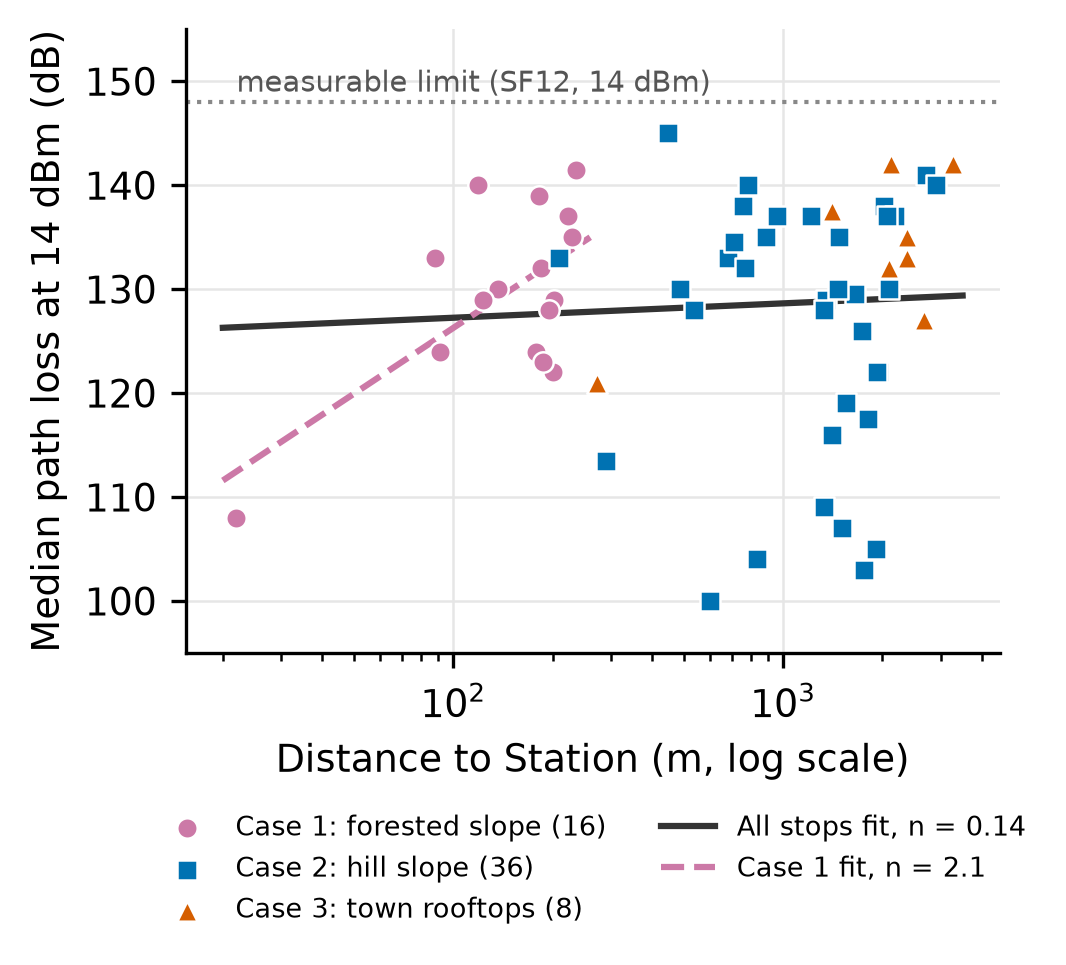
\includegraphics[width=\columnwidth]{fig1_pathloss_vs_distance.png}
\caption{Median 14\,dBm path loss against distance with log-distance fits.}
\label{fig:pl}
\end{figure}

\begin{table}[t]
\caption{Log-distance fits of median 14\,dBm path loss}\label{tab:fits}
\centering
\footnotesize
\setlength{\tabcolsep}{3pt}
\begin{tabular}{@{}lccccc@{}}
\toprule
Fit & $PL_0$ (dB) & $n$ & 95\% CI of $n$ & $R^2$ & $\sigma$ (dB) \\
\midrule
All stops (60) & 124.5 & 0.14 & $-0.44$, 0.72 & 0.00 & 11.1 \\
Case 1 (16) & 84.3 & 2.10 & 0.65, 3.56 & 0.41 & 6.7 \\
Case 2 (36) & 128.8 & $-0.07$ & $-1.66$, 1.53 & 0.00 & 12.6 \\
Case 3 (8) & 88.0 & 1.41 & $-0.15$, 2.97 & 0.45 & 5.8 \\
Tobit, all packets & 140.6 & $-0.12$ & $-1.12$, 0.64 & -- & 17.7 \\
Tobit, Case 1 & 73.2 & 3.09 & -- & -- & 12.4 \\
\bottomrule
\end{tabular}
\end{table}

\begin{figure}[t]
\centering
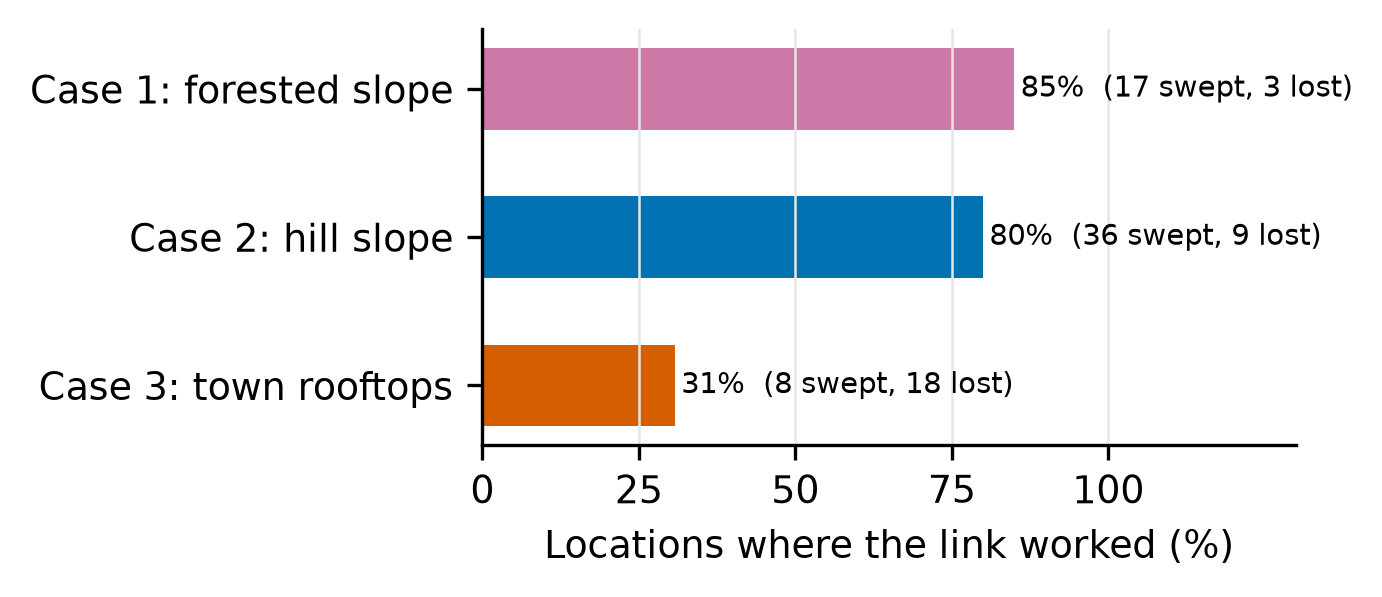
\includegraphics[width=\columnwidth]{fig8_link_success_by_case.png}
\caption{Share of attempted locations where a sweep was completed.}
\label{fig:link}
\end{figure}

\subsection{Path loss regression}
No model beat the mean-only baseline (Table~\ref{tab:reg}, Fig.~\ref{fig:rmse}). Under LOCO, terrain features raised the error to 15.0--15.8\dB, including for the random forest, against 11.4\dB for the baseline and 13.0\dB for log-distance; the largest errors occurred when Case~3 was held out. Within one case, elevation helped slightly: in Case~1 the LOO RMSE fell from 8.7 to 7.2\dB. Restricting the data to 51 stops with at least ten received packets gave the same picture. The excluded manual line-of-sight label did separate delivery (27\%, 53\% and 76\% for blocked, partly blocked and clear), which shows that path obstruction matters.

\begin{table}[t]
\caption{Path loss regression RMSE (dB)}\label{tab:reg}
\centering
\footnotesize
\setlength{\tabcolsep}{3pt}
\begin{tabular}{@{}lccc@{}}
\toprule
Model & LOO & LOCO & LOCO per case \\
\midrule
Mean only & \textbf{11.1} & \textbf{11.4} & 8.4 / 12.9 / 9.1 \\
Log-distance & 11.3 & 13.0 & 9.8 / 14.8 / 9.5 \\
+ elevation (OLS) & 11.4 & 15.8 & 11.2 / 16.3 / 20.9 \\
+ land cover (ridge) & 11.1 & 15.7 & 8.4 / 17.1 / 19.8 \\
Regression tree & 11.2 & 15.3 & 9.5 / 16.9 / 16.8 \\
Random forest & 11.3 & 15.0 & 11.8 / 16.5 / 13.0 \\
\bottomrule
\end{tabular}
\end{table}

\begin{figure}[t]
\centering
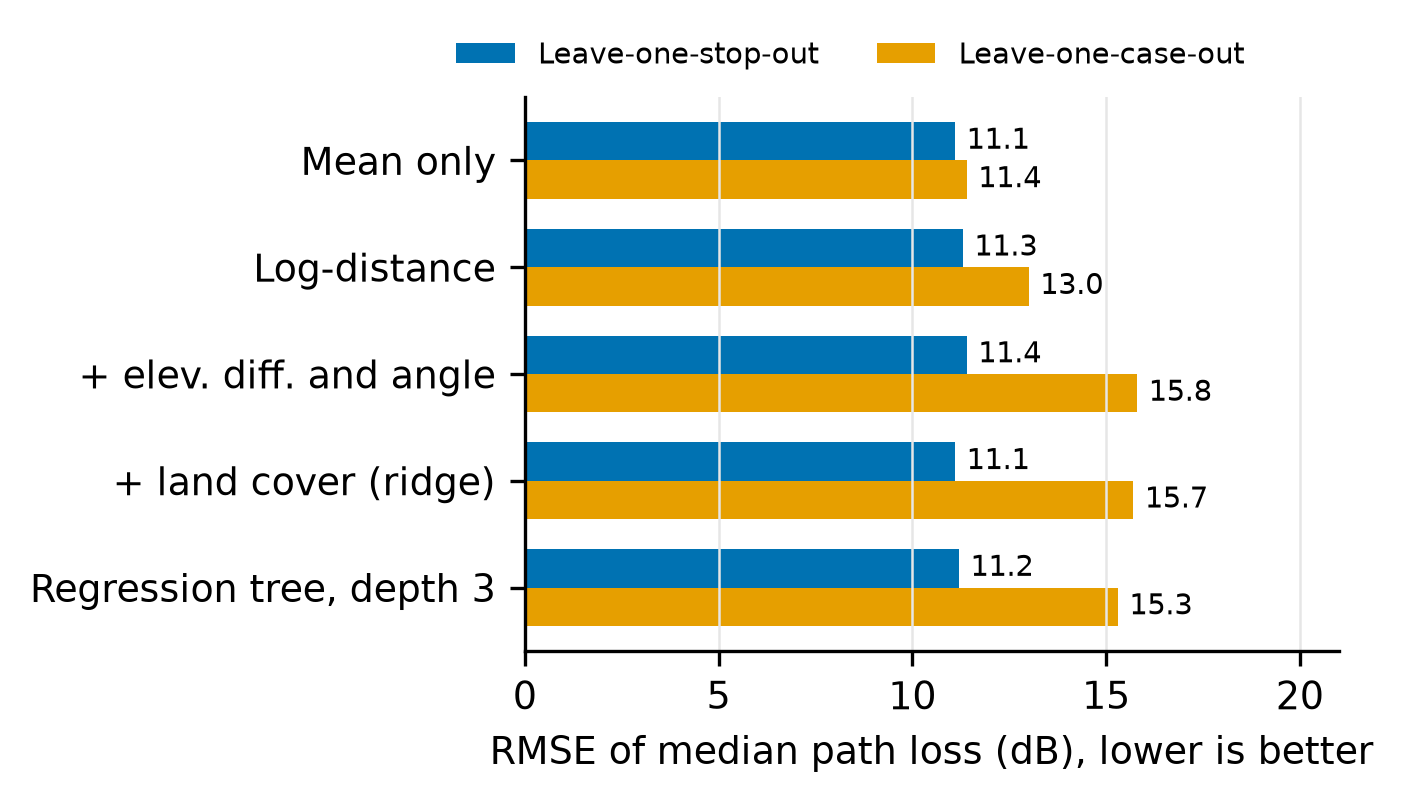
\includegraphics[width=\columnwidth]{fig4_regression_rmse.png}
\caption{Path loss RMSE under LOO and LOCO validation.}
\label{fig:rmse}
\end{figure}

\subsection{Delivery classification}
A depth-3 tree on SF and power reached a balanced accuracy of 0.68 (AUC 0.71), and 0.67 under LOCO, holding at 0.69, 0.67 and 0.72 for the held-out Cases 1--3 (Table~\ref{tab:clfmetrics}). Adding terrain features lowered LOCO to 0.50 (Fig.~\ref{fig:clf}). The random forest scored 0.89 under a random packet split but 0.65 grouped and 0.55 on an unseen case: it recognised stops rather than learning transferable rules. The tree was the most precise model (0.70); the link-budget rule predicted almost every packet as delivered (recall 0.97, precision 0.50). Gradient boosting was marginally best within known cases (AUC 0.75) but fell to 0.58 on an unseen case (Fig.~\ref{fig:roc}). Of 2,878 lost packets, the tree flagged 2,217 correctly, and it found 1,534 of 2,612 delivered ones. A learning curve rose from 0.57 with 9 training stops to 0.62--0.64 with 39--49 stops and then levelled off. The tree fitted to all data splits first on power ($\le$11\dBm): at low power, delivery is likely only when the stop lies more than about 57\,m above the Station, and at 14\dBm SF11--12 delivers most packets (Fig.~\ref{fig:tree}).

\begin{table}[t]
\caption{Delivery metrics, 10-fold grouped (threshold 0.5)}\label{tab:clfmetrics}
\centering
\footnotesize
\setlength{\tabcolsep}{2.2pt}
\begin{tabular}{@{}lccccccc@{}}
\toprule
Model & BalAcc & Prec. & Rec. & F1 & AUC & AP & LOCO \\
\midrule
Link-budget rule & 0.54 & 0.50 & 0.97 & 0.66 & 0.73 & 0.71 & -- \\
Tree, SF + power & \textbf{0.68} & \textbf{0.70} & 0.59 & 0.64 & 0.71 & 0.68 & \textbf{0.67} \\
Tree, all features & 0.62 & 0.63 & 0.53 & 0.57 & 0.64 & 0.60 & 0.50 \\
RF, all features & 0.65 & 0.63 & 0.62 & 0.63 & 0.71 & 0.66 & 0.55 \\
Logistic, SF + power & 0.68 & 0.67 & 0.64 & 0.65 & 0.73 & 0.71 & 0.65 \\
Logistic, all & 0.67 & 0.66 & 0.64 & 0.65 & 0.73 & 0.70 & 0.56 \\
Grad.\ boosting, all & 0.68 & 0.66 & 0.67 & \textbf{0.67} & \textbf{0.75} & \textbf{0.72} & 0.58 \\
\bottomrule
\end{tabular}
\end{table}

\begin{figure}[t]
\centering
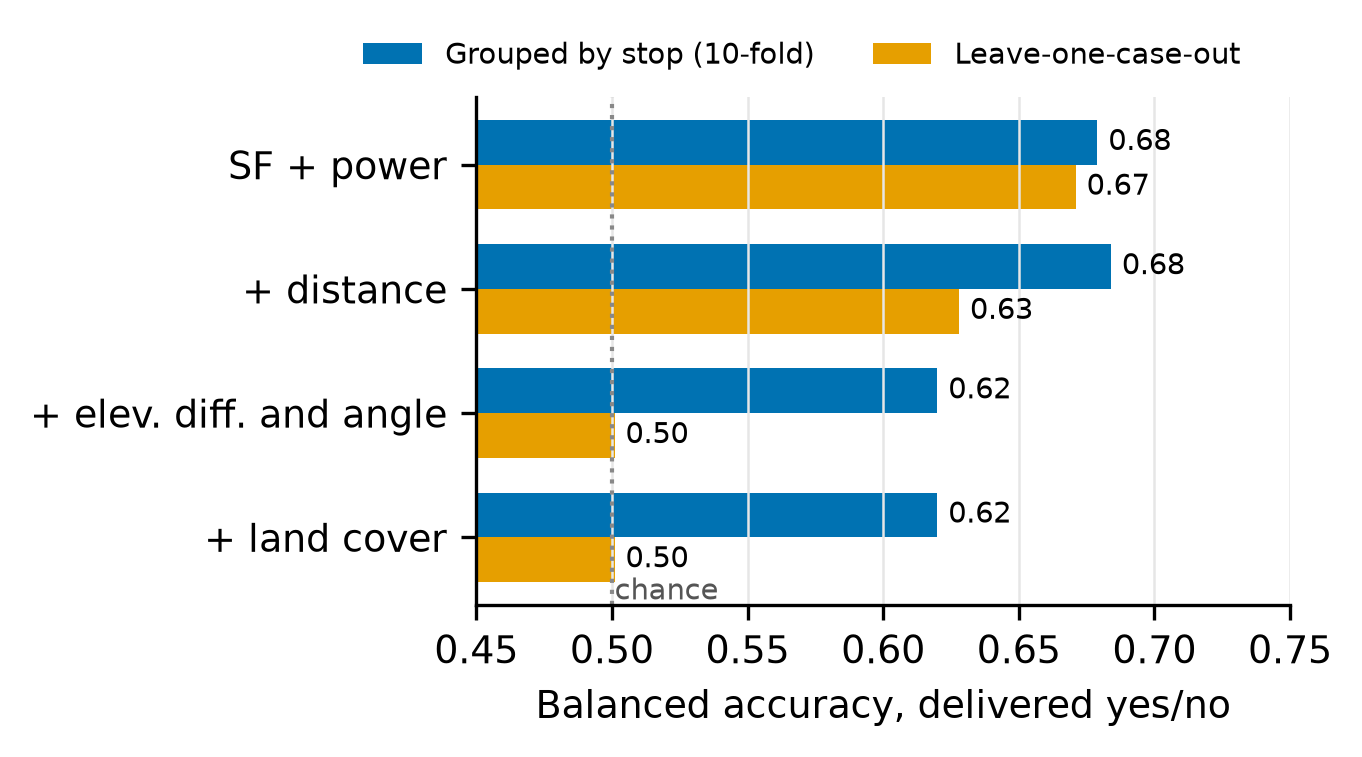
\includegraphics[width=\columnwidth]{fig5_classifier_balacc.png}
\caption{Balanced accuracy of depth-3 trees for growing feature sets.}
\label{fig:clf}
\end{figure}

\begin{figure*}[t]
\centering
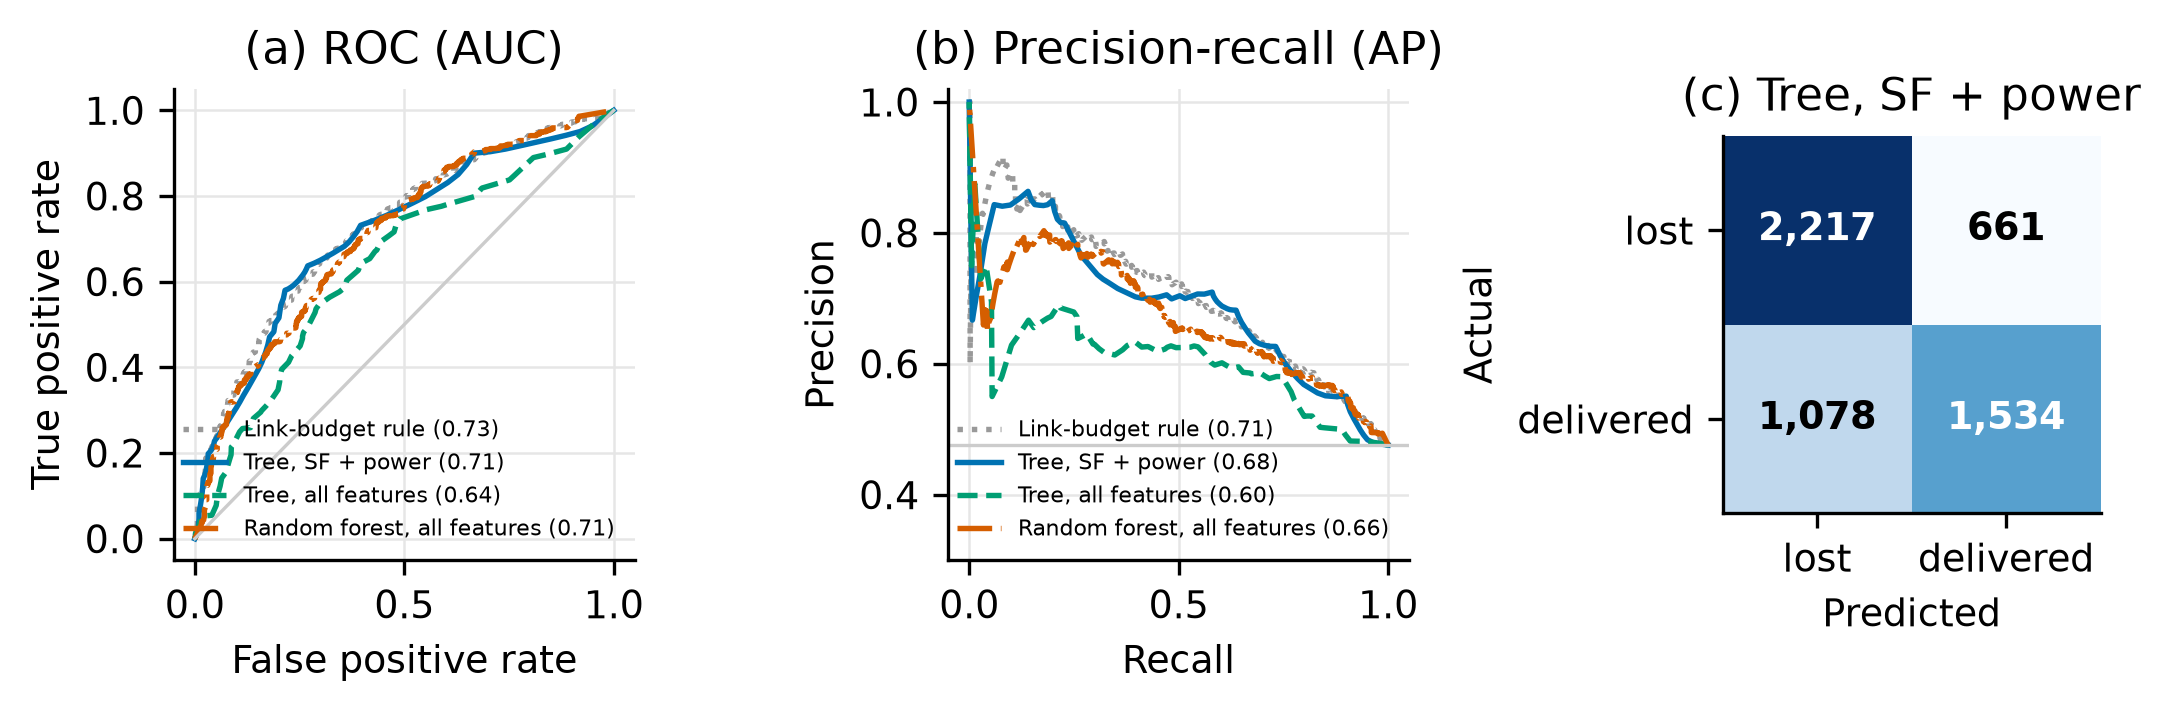
\includegraphics[width=0.92\textwidth]{fig9_roc_pr_cm.png}
\caption{(a) ROC and (b) precision--recall curves under grouped validation; (c) confusion matrix of the SF + power tree.}
\label{fig:roc}
\end{figure*}

\begin{figure*}[t]
\centering
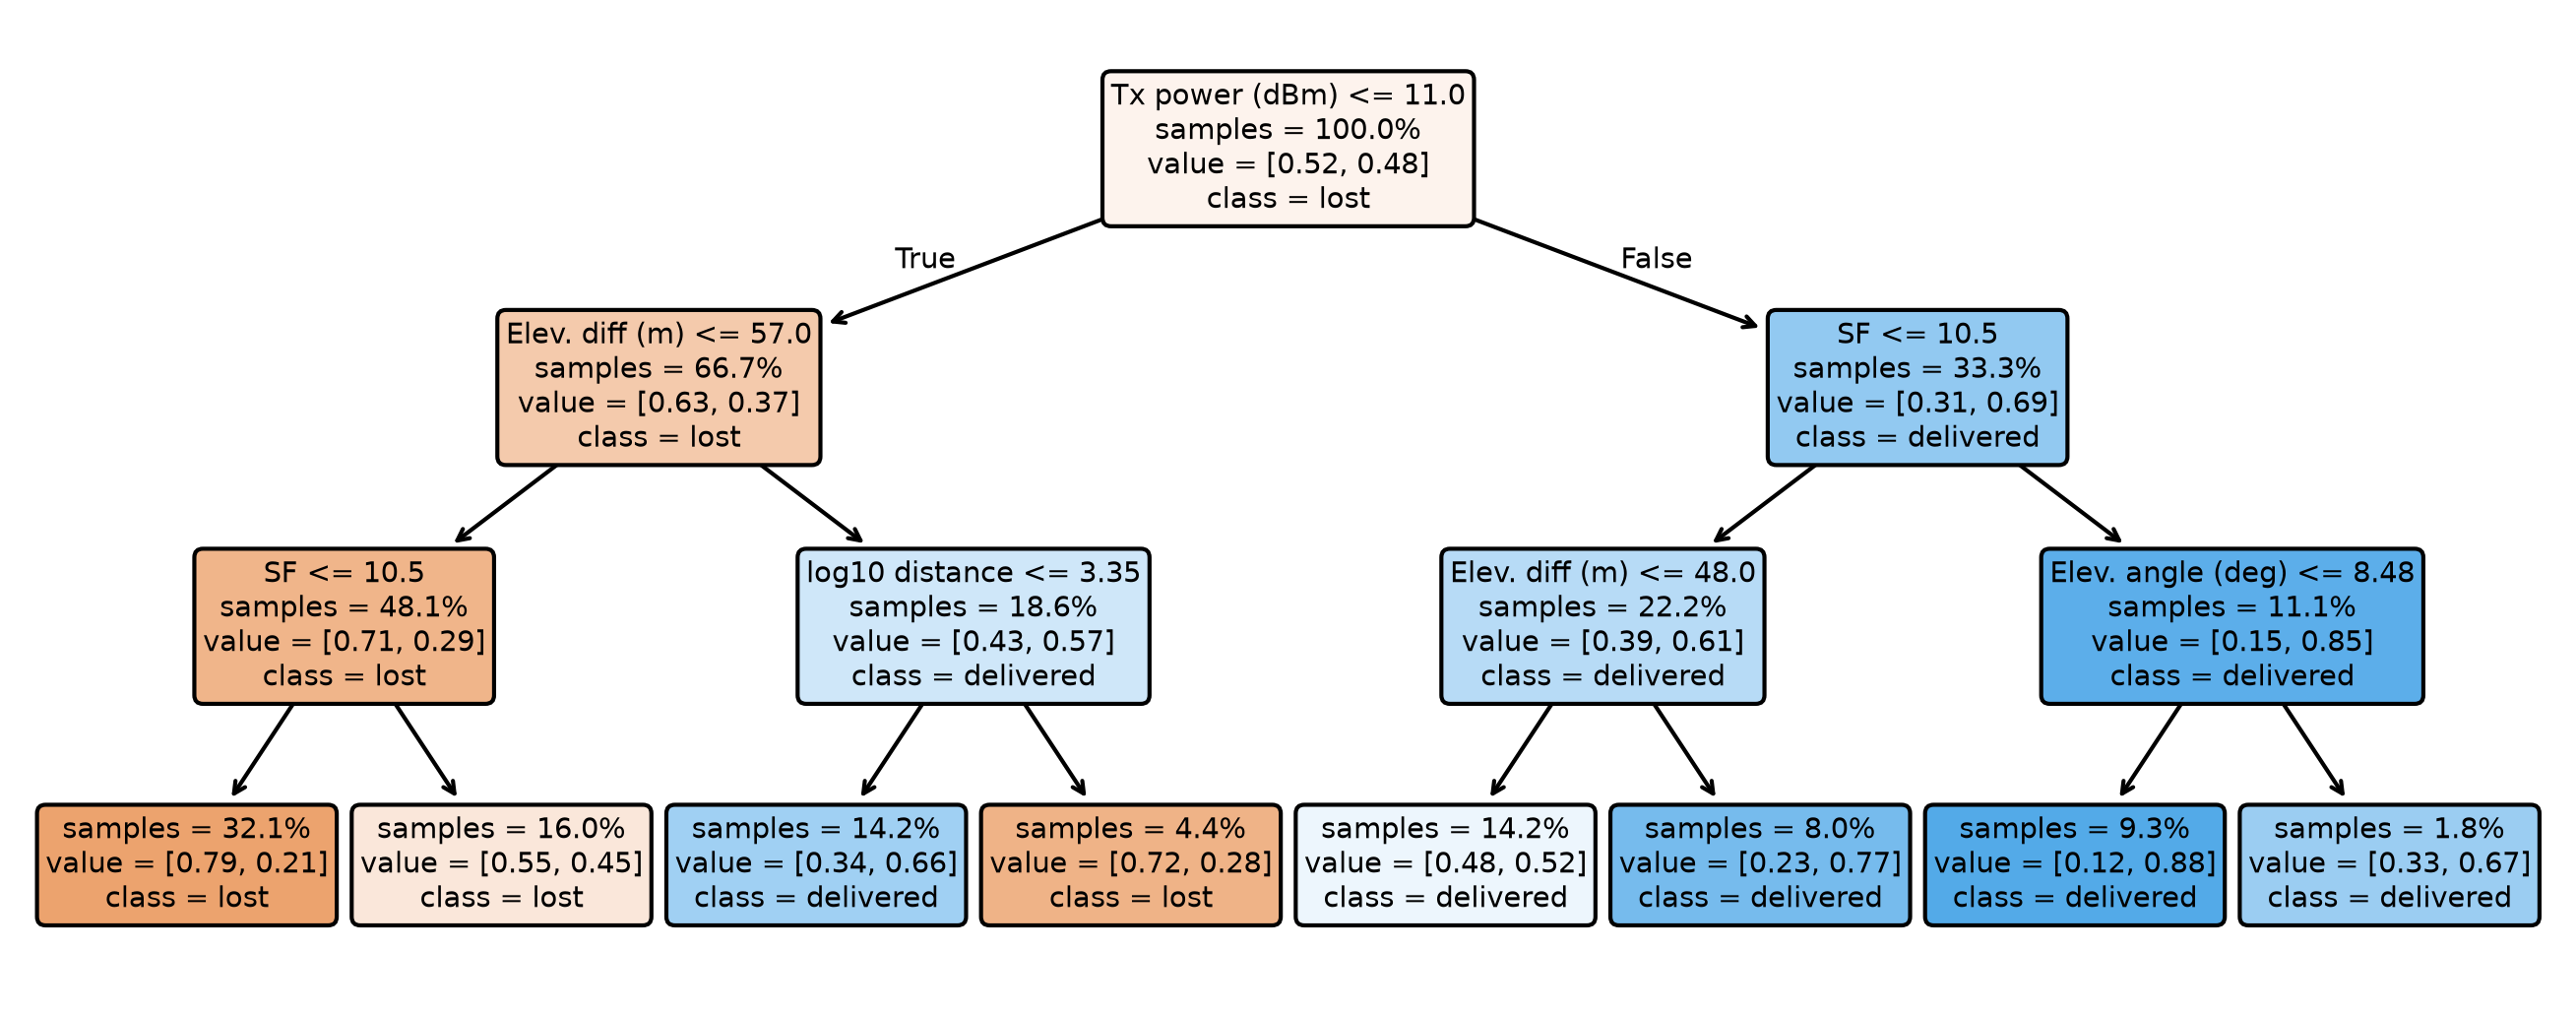
\includegraphics[width=0.9\textwidth]{fig6_tree_depth3.png}
\caption{Depth-3 delivery tree fitted to all data with all features (interpretation only).}
\label{fig:tree}
\end{figure*}

\subsection{Cheapest setting and computational cost}
At 55 of 61 stops a setting delivered at least four of five packets; 19 needed only SF9 or below at 8\dBm or below, and 7 needed SF11--12 at 14\dBm. The median stop could have used 97\% less energy than SF12 at 14\dBm (92\% in Case~3). These choices rest on five packets per setting, so they describe what was measured rather than a guaranteed long-term setting. The delivery tree trained in about 1--3\,ms and occupied about 2\,kB, whereas the forest took 0.86\,s and about 24\,MB without performing better (Table~\ref{tab:compute}).

\begin{table}[t]
\caption{Measured computational cost}\label{tab:compute}
\centering
\footnotesize
\setlength{\tabcolsep}{2.5pt}
\begin{tabular}{@{}lcrr@{}}
\toprule
Model & Complexity & Fit (ms) & Size (kB) \\
\midrule
Log-distance (OLS) & $O(nd^2)$ & 0.6 & 0.5 \\
Ridge & $O(a\,nd^2)$ & 2.2 & 1.2 \\
Regression tree & $O(d\,n\log n)$ & 0.5 & 1.7 \\
RF regressor & $O(Td\,n\log n)$ & 220 & 1,581 \\
Tobit & $O(kn)$ & 28.9 & 0.2 \\
Tree, SF + power & $O(d\,n\log n)$ & 1.2 & 2.3 \\
RF classifier & $O(Td\,n\log n)$ & 865 & 24,405 \\
\bottomrule
\end{tabular}
\end{table}

% ---------------------------------------------------------------------
\section{Discussion}\label{sec:discussion}

\begin{figure*}[!t]
\centering
\includegraphics[width=\textwidth]{fig_key_findings.png}
\caption{Key findings at a glance.}
\label{fig:keyfind}
\end{figure*}

\subsection{Answers to the research questions}
\begin{itemize}
    \item \textbf{RQ1:} Distance and endpoint terrain features did not beat the mean-only baseline; distance mattered only in Case~1 and for whether a link formed at all.
    \item \textbf{RQ2:} Radio-setting models transferred (0.67 on an unseen case); terrain-feature and more flexible models did not.
    \item \textbf{RQ3:} The cheapest setting varied widely between stops, and most stops needed far less energy than the safest setting.
\end{itemize}
Fig.~\ref{fig:keyfind} summarises these findings.

\subsection{Why distance and terrain features failed}
Three effects flatten the pooled distance trend. Censoring removes the weakest packets, although the Tobit fit shows it is not the whole story. Survivorship hides 30 mostly distant locations where no link formed. Including the lost locations, link success falls from 91\% to 52\% with distance, a trend the sweep data alone hide. Mixed terrain means distant stops across a valley can see the Station better than nearby stops behind a ridge; the positive link between delivery and stop elevation in Case~2 supports this. Endpoint features describe the two ends of a link but not the terrain between them, which matches the gains reported from path features~\cite{ojo2024,ethier2024} and the drop on held-out gateways~\cite{bitterling2026}.

\subsection{Why features did not transfer}
Within one case, terrain features helped slightly; across cases they encoded case-specific relationships and raised the error, especially for the small Case~3. A model trained where height above the Station predicted delivery (Case~2) misled it where distance mattered instead (Case~1). This is the same failure Bitterling \textit{et al.}~\cite{bitterling2026} saw when whole gateways were held out, and it is why only small, interpretable models were used.

\subsection{Was the model choice justified?}
Yes. Every flexible model lost accuracy on an unseen case, while both SF + power models kept it. The shallow tree matched the best transferable model, was the most precise, used three readable rules and was about 10,000 times smaller than the forest. Regression was the right framing for path loss, but no regression model, simple or flexible, beat the mean: the limit was the information in the features, not the model. With 61 stops, simplicity was a strength rather than a compromise.

\subsection{Comparison and practical use}
The Case~1 exponent (2.10) is close to free space, and the shadowing values (5.8--12.6\dB) are typical for outdoor LoRa. Unlike flat-terrain ranges of tens of kilometres~\cite{petajajarvi2015}, 48\% of hill locations beyond 2\,km formed no link, so a setting recommended from one link~\cite{pokharel2024} should not be reused elsewhere. The censoring-corrected Case~1 exponent (3.09) is closer to values typical of obstructed links. The larger-sample models in the literature reach 4.97 to 7.5\dB~\cite{ojo2024,ethier2024} because they describe the whole path. For practice, a planner without terrain data can expect most packets to arrive at SF11--12 and 14\dBm, but this safe setting wastes most of the energy at a typical stop. A short on-site sweep finds a much cheaper setting per node, path loss from distance alone should carry an uncertainty of about 11\dB, and the tiny tree could run on the node itself.

\subsection{Ethics and reproducibility}
No personal data were collected,. Site names and coordinates are withheld from the paper and the dashboard so that private properties cannot be located. Predictions and the dead-zone map are research outputs, not coverage guarantees for safety uses. The analysis notebook rebuilds every table and figure from the raw logs, and the dashboard reproduces the main classifier result.

% ---------------------------------------------------------------------
\section{Limitations and Future Work}\label{sec:limits}
\subsection{Limitations}
This is a small study: 61 complete stops, only eight in Case~3, from two rooftop Stations of different estimated height, all in one season. Antenna gains were not measured, so path loss is apparent rather than absolute, and rooftop heights were estimated. GPS accuracy is about 5--10\,m, SRTM resolution of 30\,m limits the elevation features, and the Station-side log was unavailable. The dead-zone map applies a model trained on 61 stops to invented terrain and is an illustration only. Results describe this area and should not be generalised beyond the three cases.

\subsection{Future work}
More stops, cases and seasons would allow firmer cross-case validation. Station-side logging and measured antenna gains would give absolute path loss. Terrain-profile features computed along each path, such as obstruction depth~\cite{ethier2024} or knife-edge diffraction loss~\cite{itu_p526}, should be tested with censoring-aware models and the same strict validation. Finally, the sweep could become an adaptive procedure in which a node tries settings from cheapest to most expensive and keeps the first that works.

% ---------------------------------------------------------------------
\section{Conclusion}\label{sec:conclusion}
Across 61 stops in three hill-terrain cases, delivery was governed by spreading factor and power, and a shallow tree on these two settings kept its accuracy on an unseen case while being among the cheapest models. More flexible models, including random forests and gradient boosting, did not transfer better. Path loss could not be predicted from distance or endpoint terrain better than by its mean (RMSE 11.1\dB), and a log-distance model held only in the short-range obstructed case. Per-stop settings could save a median 97\% of transmit energy. Receiver censoring, unrecorded failed links and terrain mixing explain much of this. In hill terrain, what lies between the antennas matters more than the distance between them.

\section*{Acknowledgment}
I thank my module tutors at Softwarica College of IT and E-Commerce for their guidance and feedback. Generative AI tools assisted with code, figure layout and language editing; the experiment design, field measurements, analysis decisions and conclusions are my own, and every reported number was checked against the analysis notebook.

\section*{Data Availability}
The raw Roamer logs, stop features, analysis notebook and dashboard code are available from the author on request. Site names and exact locations are withheld.

% ---------------------------------------------------------------------
\begin{thebibliography}{00}

\bibitem{rappaport2002}
T.~S. Rappaport, \emph{Wireless Communications: Principles and Practice}, 2nd~ed. Upper Saddle River, NJ, USA: Prentice Hall, 2002.

\bibitem{hata1980}
M.~Hata, ``Empirical formula for propagation loss in land mobile radio services,'' \emph{IEEE Trans. Veh. Technol.}, vol.~29, no.~3, pp.~317--325, 1980.

\bibitem{itu_p526}
ITU-R, ``Propagation by diffraction,'' Recommendation ITU-R P.526, International Telecommunication Union, Geneva, Switzerland.

\bibitem{petajajarvi2015}
J.~Petäjäjärvi, K.~Mikhaylov, A.~Roivainen, T.~Hänninen, and M.~Pettissalo, ``On the coverage of LPWANs: Range evaluation and channel attenuation model for LoRa technology,'' in \emph{Proc. 14th Int. Conf. ITS Telecommunications (ITST)}, 2015, doi:10.1109/ITST.2015.7377400.

\bibitem{rademacher2021}
M.~Rademacher, H.~Linka, T.~Horstmann, and M.~Henze, ``Path loss in urban LoRa networks: A large-scale measurement study,'' \emph{arXiv preprint arXiv:2109.07768}, 2021.

\bibitem{bianco2020}
G.~M. Bianco, A.~Mejia-Aguilar, and G.~Marrocco, ``Radio wave propagation of LoRa systems in mountains for search and rescue operations,'' in \emph{Proc. URSI General Assembly and Scientific Symposium (URSI GASS)}, 2020.

\bibitem{pokharel2024}
A.~Pokharel, P.~Sapkota, D.~Sapkota, S.~Dahal, S.~Karki, and R.~K. Budhathoki, ``Performance evaluation of LoRa technology for rural connectivity: An experimental analysis in Nepal,'' \emph{arXiv preprint arXiv:2412.04563}, 2024.

\bibitem{bitterling2026}
R.~Bitterling, C.~Nettersheim, J.~Hees, and M.~Rademacher, ``A systematic sample size analysis of ML-based path loss prediction for LPWAN,'' \emph{arXiv preprint arXiv:2608.11083}, 2026.

\bibitem{breiman2001}
L.~Breiman, ``Random forests,'' \emph{Machine Learning}, vol.~45, no.~1, pp.~5--32, 2001, doi:10.1023/A:1010933404324.

\bibitem{breiman1984}
L.~Breiman, J.~H. Friedman, R.~A. Olshen, and C.~J. Stone, \emph{Classification and Regression Trees}. Belmont, CA, USA: Wadsworth, 1984.

\bibitem{ojo2024}
M.~O. Ojo, I.~Viola, S.~Miretti, E.~Martignani, S.~Giordano, and M.~Baratta, ``A deep learning approach for accurate path loss prediction in LoRaWAN livestock monitoring,'' \emph{Sensors}, vol.~24, no.~10, p.~2991, 2024, doi:10.3390/s24102991.

\bibitem{tobin1958}
J.~Tobin, ``Estimation of relationships for limited dependent variables,'' \emph{Econometrica}, vol.~26, no.~1, pp.~24--36, 1958.

\bibitem{gustafson2015}
C.~Gustafson, T.~Abbas, D.~Bolin, and F.~Tufvesson, ``Statistical modeling and estimation of censored pathloss data,'' \emph{arXiv preprint arXiv:1504.03977}, 2015.

\bibitem{roberts2017}
D.~R. Roberts \emph{et al.}, ``Cross-validation strategies for data with temporal, spatial, hierarchical, or phylogenetic structure,'' \emph{Ecography}, vol.~40, no.~8, pp.~913--929, 2017, doi:10.1111/ecog.02881.

\bibitem{ethier2024}
J.~Ethier and M.~Châteauvert, ``Machine learning-based path loss modeling with simplified features,'' \emph{arXiv preprint arXiv:2405.10006}, 2024.

\bibitem{semtech_an1200}
Semtech Corporation, ``LoRa modulation basics,'' Application Note AN1200.22, 2015.

\bibitem{augustin2016}
A.~Augustin, J.~Yi, T.~Clausen, and W.~M. Townsley, ``A study of LoRa: Long range \& low power networks for the Internet of Things,'' \emph{Sensors}, vol.~16, no.~9, p.~1466, 2016, doi:10.3390/s16091466.

\bibitem{nta2023}
Nepal Telecommunications Authority, ``Radio Frequency Policy,'' Kathmandu, Nepal, 2023.

\bibitem{farr2007}
T.~G. Farr \emph{et al.}, ``The Shuttle Radar Topography Mission,'' \emph{Rev. Geophys.}, vol.~45, no.~2, RG2004, 2007, doi:10.1029/2005RG000183.

\bibitem{pedregosa2011}
F.~Pedregosa \emph{et al.}, ``Scikit-learn: Machine learning in Python,'' \emph{J. Mach. Learn. Res.}, vol.~12, pp.~2825--2830, 2011.

\end{thebibliography}

% ---------------------------------------------------------------------
\appendices
\section{Field use and analysis notebook}\label{app:hw}
Fig.~\ref{fig:hardware} shows the Roamer carried during the field walk and its interface after a sweep, which displays delivery for each SF and power. Figs.~\ref{fig:nb-data}--\ref{fig:nb-cost} are excerpts of the executed analysis notebook. They cover data loading and checks, path loss regression, the delivery classifiers and the cost measurements. Cells printing GPS coordinates are omitted.

\begin{figure*}[t]
\centering
\begin{subfigure}[t]{0.45\textwidth}\centering\photo{roamer_bag.jpg}\caption{Roamer carried in a bag}\end{subfigure}\hfill
\begin{subfigure}[t]{0.45\textwidth}\centering\photo{packet_screen.jpg}\caption{Roamer interface after a sweep}\end{subfigure}
\caption{Field use of the Roamer.}
\label{fig:hardware}
\end{figure*}

\begin{figure*}[p]
\centering
\includegraphics[width=0.9\textwidth]{nb_appendix_data.png}
\caption{Notebook: combining the site logs and data checks.}
\label{fig:nb-data}
\end{figure*}

\begin{figure*}[p]
\centering
\includegraphics[width=0.9\textwidth]{nb_appendix_regression.png}
\caption{Notebook: path loss regression.}
\label{fig:nb-reg}
\end{figure*}

\begin{figure*}[p]
\centering
\includegraphics[width=0.9\textwidth]{nb_appendix_classification.png}
\caption{Notebook: delivery classifiers, metrics, ROC and confusion matrix.}
\label{fig:nb-clf}
\end{figure*}

\begin{figure*}[p]
\centering
\includegraphics[width=0.9\textwidth]{nb_appendix_cost.png}
\caption{Notebook: cheapest setting and computational cost.}
\label{fig:nb-cost}
\end{figure*}

\section{Interactive dashboard}\label{app:dash}
Fig.~\ref{fig:dash} shows the Gradio dashboard. It has seven tabs: overview, delivery explorer, path loss, model results, a model lab, the dead-zone map, and method and limits. It reads the raw logs with relative paths, removes coordinates, and runs locally or in Google Colab. The model lab reproduces the SF + power tree result live (balanced accuracy 0.68, AUC 0.71, LOCO 0.67). The dead-zone map is an illustration on synthetic terrain: where the tree's prediction and the line-of-sight layer disagree marks the information that endpoint features cannot capture.

\begin{figure*}[t]
\centering
\begin{subfigure}[t]{0.49\textwidth}\centering\includegraphics[width=\linewidth]{dash_overview.jpg}\caption{Overview}\end{subfigure}\hfill
\begin{subfigure}[t]{0.49\textwidth}\centering\includegraphics[width=\linewidth]{dash_deadzone3d.jpg}\caption{Dead-zone map, 3-D view}\end{subfigure}
\caption{Gradio dashboard (no site names or coordinates).}
\label{fig:dash}
\end{figure*}

\end{document}
